\section{Arquitectura general}

La Figura \ref{fig:arquitectura-open-glove}, muestra un diagrama conceptual general de OpenGlove, donde es posible ver el trabajo previo realizado por \cite{tesis-monsalve-rodrigo}, \cite{tesis-meneses-sebastian} y \cite{tesis-cerda-rodrigo}, como también el trabajo que resulta de este proyecto y el que se realizará en un futuro.

\begin{figure}[H]
  \begin{center} 
   	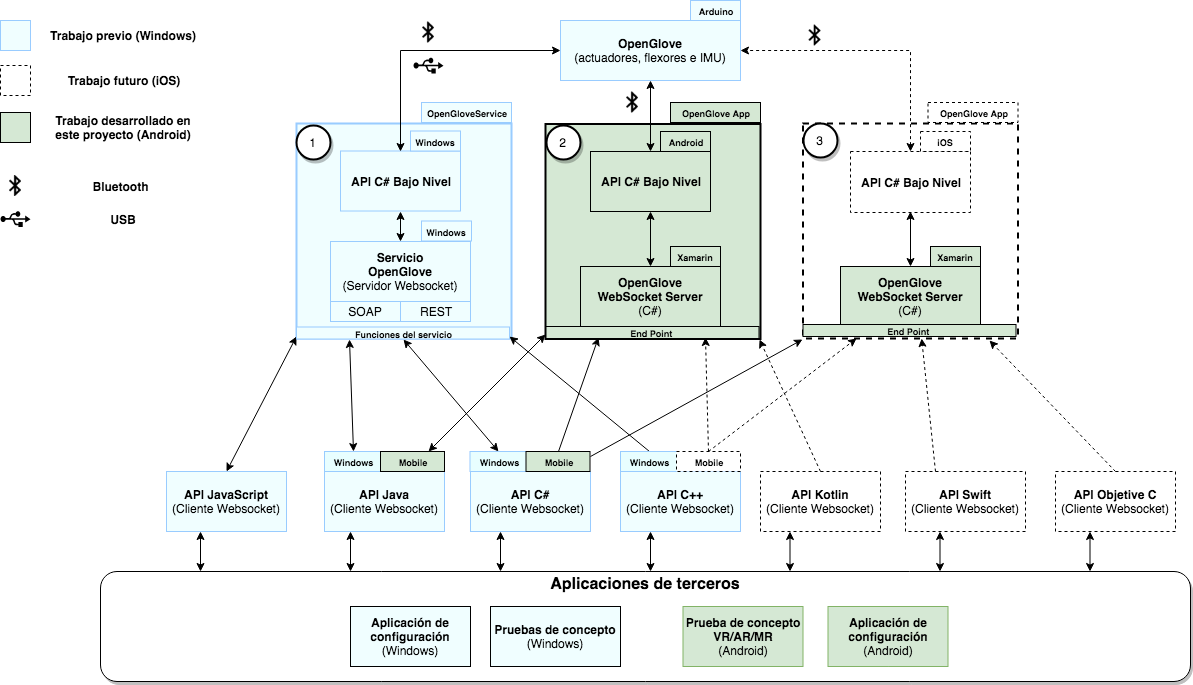
\includegraphics[width=1.0\textwidth]{images/chapter04/OpenGlove-Architecture-General.png} 
    \caption[Diagrama conceptual general de OpenGlove]{Diagrama conceptual general de OpenGlove \\Fuente: Elaboración propia (2018)}
    \label{fig:arquitectura-open-glove}
  \end{center}
\end{figure}

La aplicación de configuración de OpenGlove desarrollada en este proyecto, permite comunicarse con dispositivos OpenGlove a través de comunicación serial Bluetooth. Para acceder a sus funcionalidades los desarrolladores hacen uso de las APIs de alto nivel, las cuales corresponden a clientes WebSocket. Éstas pueden ser utilizadas en cualquier aplicación compatible con el lenguaje de la API a utilizar. Dado que se utiliza Xamarin.Forms para desarrollar aplicaciones nativas multiplataforma, para iOS y Android, el servidor Websocket es desarrollado utilizando bibliotecas de software de C\#, para que ambas plataformas compartan el código. La API de bajo nivel, debe ser específica en cada sistema operativo, por las diferencias de comunicación presentes en cada uno. Por esta misma razón se desarrollan las APIs de alto nivel en  Java y C\#. La primera permite hacer uso de OpenGlove en proyectos Android y la segunda permite hacer aplicaciones para iOS y Android utilizando Xamarin. El uso de Xamarin.Forms permite reutilizar código de la Interfaz de Usuario y desarrollar de manera específica para cada plataforma utilizando un mismo lenguaje de programación. Cabe destacar que la comunicación realizada entre las APIs y la aplicación es mediante WebSockets considerando que OpenGlove es una aplicación que transmite datos en tiempo real.

\begin{figure}[H]
  \begin{center} 
   	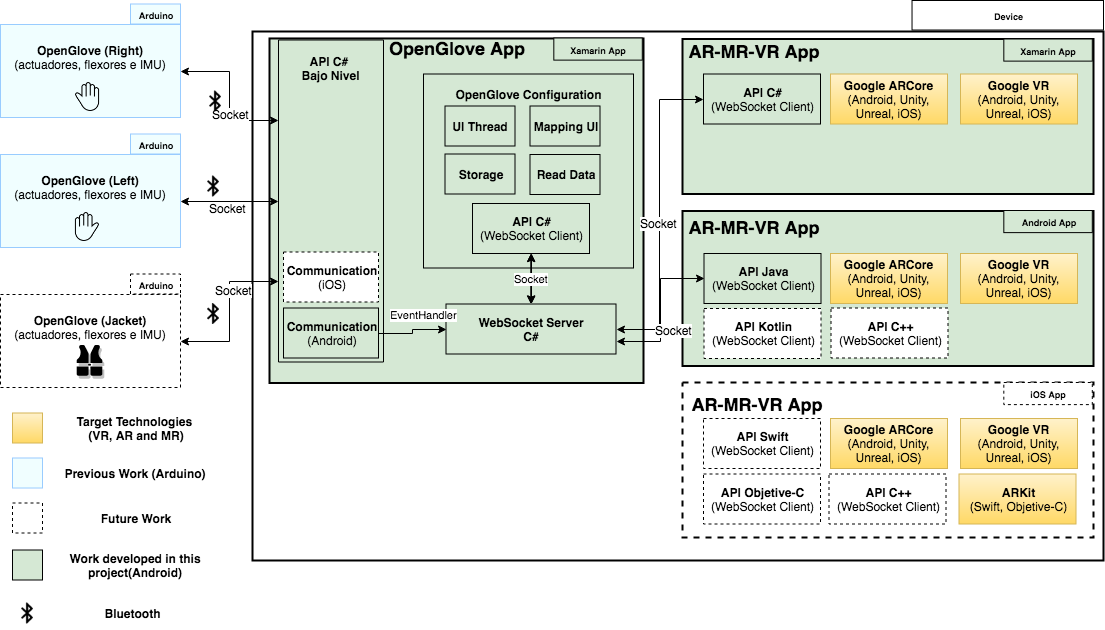
\includegraphics[width=1.0\textwidth]{images/chapter04/OpenGlove-Architecture-Specification.png} 
    \caption[Detalle Arquitectura de Openglove]{Detalle Arquitectura de OpenGlove \\Fuente: Elaboración propia (2018)}
    \label{fig:detalle-arquitectura-open-glove}
  \end{center}
\end{figure}

La Figura \ref{fig:detalle-arquitectura-open-glove} muestra un diagrama conceptual de la arquitectura en detalle, donde se consideró el objetivo de uso de las APIs de alto nivel en Java y C\#. Las APIs de alto nivel mencionadas permiten el desarrollo de aplicaciones de terceros en Android nativo usando Java o con C\# utilizando Xamarin. Para realizar aplicaciones de AR o VR, se puede utilizar Google ARCore y Google VR respectivamente. Ambas herramientas de Google están disponibles para Android, iOS, Unity y Unreal.

Esta arquitectura establece al servidor WebSocket como punto de acceso a las funcionalidades referentes a los actuadores, flexores e IMU. Por tanto la aplicación de configuración y las aplicaciones de terceros utilizan las mismas APIs de alto nivel para su desarrollo, evitando replicación de código y aprovechando todas las funcionalidades provistas por la API de alto nivel. La aplicación de configuración de OpenGlove desarrollada en Xamarin.Forms, utiliza la API de alto nivel C\#.

Dado el alcance de la solución, no se ha desarrollado APIs de alto nivel que tengan como objetivos aplicaciones de terceros para iOS, para lo cual requiere un dispositivo iPhone real para realizar las pruebas de Bluetooth y WebSockets, o en su defecto un MacBook para poder visualizar la interfaz de la aplicación, pero sin hacer uso de las funcionalidades Bluetooth ni WebSocket. También es importante recalcar la necesidad de implementar parte de la API de bajo nivel en C\# ( Communication ) específica para iOS para gestionar las conexiones de los dispositivos Bluetooth y la administración de mensajes entre la API de bajo nivel y el servidor WebSocket. Este es un trabajo que se puede realizar a futuro para dar soporte a OpenGlove en iOS.


